\documentclass[journal]{IEEEtran}
%\documentclass[a4paper, 10pt, conference]{ieeeconf}      % Use this line for a4
                                                         % paper
\IEEEoverridecommandlockouts        % This command is only
% needed if you want to
                                    % use the \thanks command
%\overrideIEEEmargins
% See the \addtolength command later in the file to balance the column lengths
% on the last page of the document
% The following packages can be found on http:\\www.ctan.org
\usepackage{graphics} % for pdf, bitmapped graphics files
\usepackage{rotating} % rotate figures
\usepackage{epsfig} % for postscript graphics files
%\usepackage{mathptmx} % assumes new font selection scheme installed
%\usepackage{times} % assumes new font selection scheme installed
\usepackage{amsmath}
\usepackage{amssymb}
\usepackage[spanish]{babel}
\usepackage{cite}

\usepackage{atbegshi} % erase first blank page
\usepackage{hyperref}

\AtBeginDocument{\AtBeginShipoutNext{\AtBeginShipoutDiscard}}

\title{\LARGE \bf Proyecto de Aprendizaje por Refuerzo}

%%%%%%%%%%%%%%%%%%%%%% AUTHORS %%%%%%%%%%%%%%%%%%%%%%%%%%%%%%%%%%%%%%%%5
\author{Juan Pablo Echeagaray González, Emily Rebeca Méndez Cruz, Grace Aviance Silva Arostegui}% <-this % stops 
\begin{document}

    \thanks{Juan Pablo Echeagaray González, Emily Rebeca Méndez Cruz, Grace Aviance Silva Arostegui pertencen al Tec de Monterrey campus Monterrey, N.L. C.P. 64849, Mexico {\tt\small}}

    \maketitle

    \thispagestyle{empty}
    \pagestyle{empty}
    
    \begin{abstract}
        Se realizó una comparación del desempeño de 4 modelos de aprendizaje no supervisado, se comparó el tiempo de entrenamiento y el puntaje silhouette. Encontramos que el mejor modelo para la base de datos fue el spectral clustering.
    \end{abstract}

    \begin{IEEEkeywords} 
    Data Science, Machine Learning, Reinforcement Learning
    \end{IEEEkeywords}

    %%%%%%%%%%%%%%%%%%%%%%%%%%%%%%%%%%%%%%%%%%%%%%%%%%%%%%%%%%%%%%%%%%%%%%%%%%%%%%%%
    \section{Introducción} \label{introduction}

        La base de datos fue recuperada de Kaggle (la liga de acceso se encuentra en el apéndice \ref{data}), para nuestro caso de estudio hemos escogido una base de datos enfocada en la clasificación de riesgo para el cáncer cervical.

        La información que contiene son  857 registros de mujeres en las que se les identifica datos, características y/o enfermedades significativas para incrementar el riesgo para contraer cáncer cervical. Entre ellos: la edad, el número de parejas sexuales, la edad de la primera relación sexual, número de embarazos, si fuma o no, el número de años fumando, el número de cajetillas consumidas por año, si consumen o no anticonceptivos, el número de años consumiendo anticonceptivos, si usan o no DIU, el número de años usando DIU, si tienen ETS o no, el número de ETS que tienen, si tienen o no los siguientes tipos de ETS (condilomatosis, condilomatosis cervical, condilomatosis vaginal, condilomatosis vulvo-perineal, sífilis, enfermedad inflamatoria pélvica, herpes, molusco contagioso, AIDs, VIH, hepatitis B, HPV, número de diagnósticos, tiempo desde el primer diagnóstico, tiempo del último diagnóstico), cáncer, CIN, HPV, Hinselmann, Schiller, citología, y biopsia.

        Las columnas de la base de datos Hinselmann, Schiller, citología, y biopsia, son variables binarias que representan diferentes estudios que tratan de encontrar cáncer en el cuello utirino de las pacientes. Dada la documentación de la base de datos, no nos fue posible determinar cuál de estos 4 estudios es el más fiable para la determinación de la presencia de un cáncer, por lo que hemos optado por la creación de una nueva variable se define como la suma de los valores que toman los estudios en la base de datos, esto resulta en una variable con 5 posibles valores, un mínimo de 0 representando un riesgo nulo o bajo de tener cáncer, y un valor máximo de 4 representando el mayor riesgo de tenerlo.

        El objetivo de nuestro proyecto es diseñar un modelo de \emph{Aprendizaje por Refuerzo} que agrupe de forma exitosa a los pacientes presentes en la base de datos.

    \section{Créditos} \label{credits}
       
        \begin{itemize}
            \item Juan Pablo Echeagaray González - Data Scientist
            \item Emily Rebeca Méndez Cruz - Data Scientist
            \item Grace Aviance Silva Aróstegui - Data Scientist
        \end{itemize}

    \section{Modelos de Aprendizaje por Refuerzo} \label{modelos}
        
        \vspace*{3mm}
        \subsection{K-Means - Grace Aviance Silva Arostegui} \label{kmeans}
        
        Es un algoritmo de clustering no supervisado de gran popularidad por su velocidad y simplicidad. También es conocido como \textit{geometric clustering algorithm}. El enfoque detrás de este algoritmo simple se trata solo de algunas iteraciones y la actualización de grupos según las medidas de distancia que se calculan repetidamente. k es el número de conglomerados que se van a formar.
            
            \vspace*{2mm}
            \subsubsection{Objetivo}
            
            El objetivo de este algoritmo es agrupar los datos de entrada en en K clases distintas. El algoritmo se basa en definir K centroides en el espacio dimensional de los datos de entrada, e iterativamente ajustar sus posiciones. Como resultado se consigue dividir el espacio de los datos en  K celdas de Voronoi (uno por centroide), pudiendo asociar cada observación de entrada al centroide más cercano. \cite{datacamp}
            
            \vspace*{2mm}
            \subsubsection{Implementación}
            
                Para nuestra implementación utilizamos la librería scikit-learn, a través de su API importamos las funciones KMeans, make blobs,  silhouette score, y, StandardScaler.
                
                En términos básicos, esta organizado este algoritmo en 3 pasos. \cite{kmeans} 
                \begin{itemize}
                    \item El primer paso elige los centroides iniciales, con el método más básico para elegir \textit{k} muestras del conjunto de datos \textit{X}. Después de la inicialización, K-means consiste en un bucle entre los otros dos pasos. Este primer paso asigna cada muestra a su centroide más cercano.
                    \item El segundo paso crea nuevos centroides tomando el valor medio de todas las muestras asignadas a cada centroide previamente. 
                    \item Se repetirá esto hasta que los centroides no tengan una posición más significativa para moverse
                \end{itemize}
                
                \begin{figure}[h]
                    \centering
                    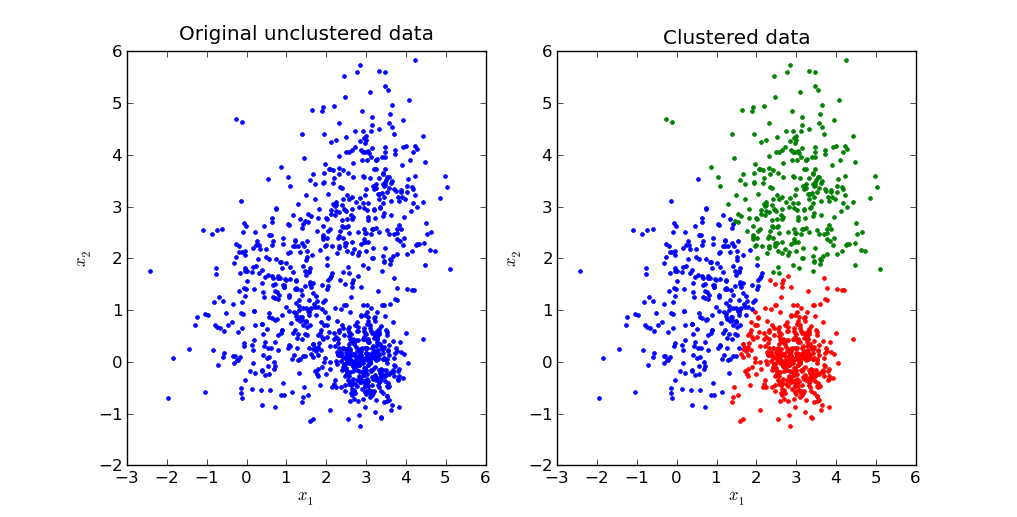
\includegraphics[scale=0.38]{img/kmeans.png}
                \end{figure}
 
            
        \subsection{Dendograma - Emily Rebeca Méndez Cruz} \label{dendrogram}
        
            El dendrograma es un diagrama de árbol que muestra los grupos que se forman al crear conglomerados de observaciones en cada paso y sus niveles de similitud, es decir,  expone las distancias de atributos entre cada par de clases fusionadas de manera secuencial. El nivel de similitud se mide en el eje vertical y las diferentes observaciones se especifican en el eje horizontal \cite{minitab}. Para evitar cruzar líneas, el diagrama se expone gráficamente de tal modo que los miembros de cada par de clases que se fusionan son elementos próximos ,\cite{desktop}.
            Se utiliza para observar cómo se forman los conglomerados en cada paso y para evaluar los niveles de similitud (o distancia) de los conglomerados que se forman \cite{minitab}. 
            
            \begin{figure}[h!]
                \centering
                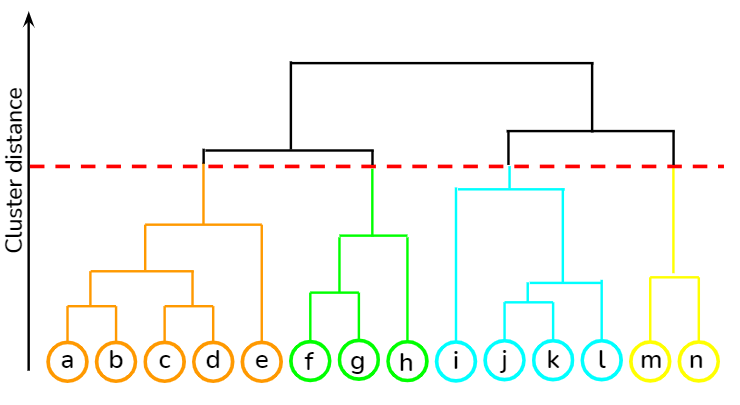
\includegraphics[width=7cm]{img/dendrograma.png}
                \caption{Ejemplo de dendrograma}
            \end{figure}
    
            \subsubsection{Objetivo}
            
                El principal objetivo es realizar un número óptimo de grupos y asignar objetos a los grupos, esto con el fin de de generar un conjunto de agrupaciones que logre juntar las posibles diferencias entre los pacientes.
            
            \subsubsection{Implementación}
            
            Para el dendrograma se hizo uso del paquete plotly.figure\_factory, este contiene funciones dedicadas para crear tipos muy específicos de gráficos, el cual para nuestro caso es el dendrograma. Donde nuestros parámetros son:
            
            \begin{itemize}
            \item X
            \item Color\_threshold
            \item Orientation
            \end{itemize}

        
        \subsection{Spectral Clustering - Juan Pablo Echeagaray González} \label{spectral}
        
            Este algoritmo recibe de base (normalmente) una matriz de similitud entre un conjunto de instancias y produce una representación en un espacio dimensional menor, en otras palabras, realiza un proceso de reducción de dimensionalidad. Una vez que se está en este espacio, ajusta un modelo de agrupamiento, para el caso de \emph{sci-kit learn} se usa \emph{k-means} \cite{geron2019hands}.
            
            \subsubsection{Objetivo}
                
                Para este caso, hemos de entrenar un modelo de esta clase para reducir la dimensionalidad de los datos y agrupar a todos los pacientes en diferentes clases, esperamos que como resultado se encuentre una distribución correcta de los distintos niveles de riesgo de contraer cáncer.
                
            \vspace*{2mm}    
            \subsubsection{Implementación}
            
                En este caso, el parámetro \emph{gamma} que representa el coeficiente usado por el kernel. De diferentes pruebas hemos encontrado que el mejor desempeño del modelo ocurre cuando \emph{gamma} toma el valor de 0.01.
                
            \begin{figure}[ht]
                \centering
                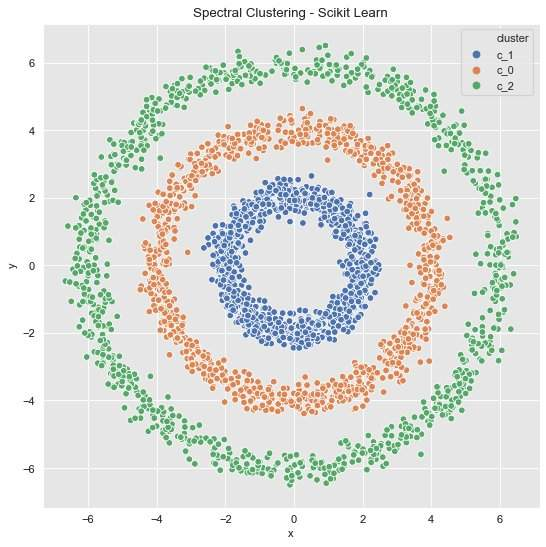
\includegraphics[scale=0.38]{img/spectral.jpg}
            \end{figure}
                
        \subsection{DBSCAN - Juan Pablo Echeagaray González} \label{DBSCAN}

            DBSCAN es otro algoritmo de agrupamiento no supervisado. De forma general, este algoritmo define \emph{clusters} como regiones continuas con alta densidad (es decir, que contengan muchas instancias).

            \subsubsection{Algoritmo}

                El libro \emph{Hands-on machine learning with Scikit-Learn, Keras, and TensorFlow: Concepts, tools, and techniques to build intelligent systems} brinda una excelente descripción de su funcionamiento en un nivel general, además de enseñar cómo utilizarlo en \emph{Python} \cite{geron2019hands}.

                \begin{enumerate}
                    \item Para cada instancia, determinar cuántas instancias más están lo suficientemente cerca de el (controlado por un parámetro $\epsilon$). La región obtenida se conoce como el \emph{vecindario-$\epsilon$}.
                    \item Si el objeto tiene al menos un cierto número de instancias (\emph{min\_samples}) en su \emph{vecindario-$\epsilon$}, entonces se le considera como una instancia núcleo. Dicho de otra manera, estas instancias se ubican en las regiones densas.
                    \item Todas las instancias que estén dentro de la región de una instancia núcleo pertenecen al mismo clúster. En este proceso se pueden llegar a incluir más instancias núcleo formando grandes cadenas que seguirán formando parte del mismo clúster.
                    \item Al finalizar este proceso, cualquier instancia que no sea una instancia núcleo o que no esté dentro de un vecindario, será considerada como una anomalía.
                \end{enumerate}
                
                \begin{figure}[ht]
                    \centering
                    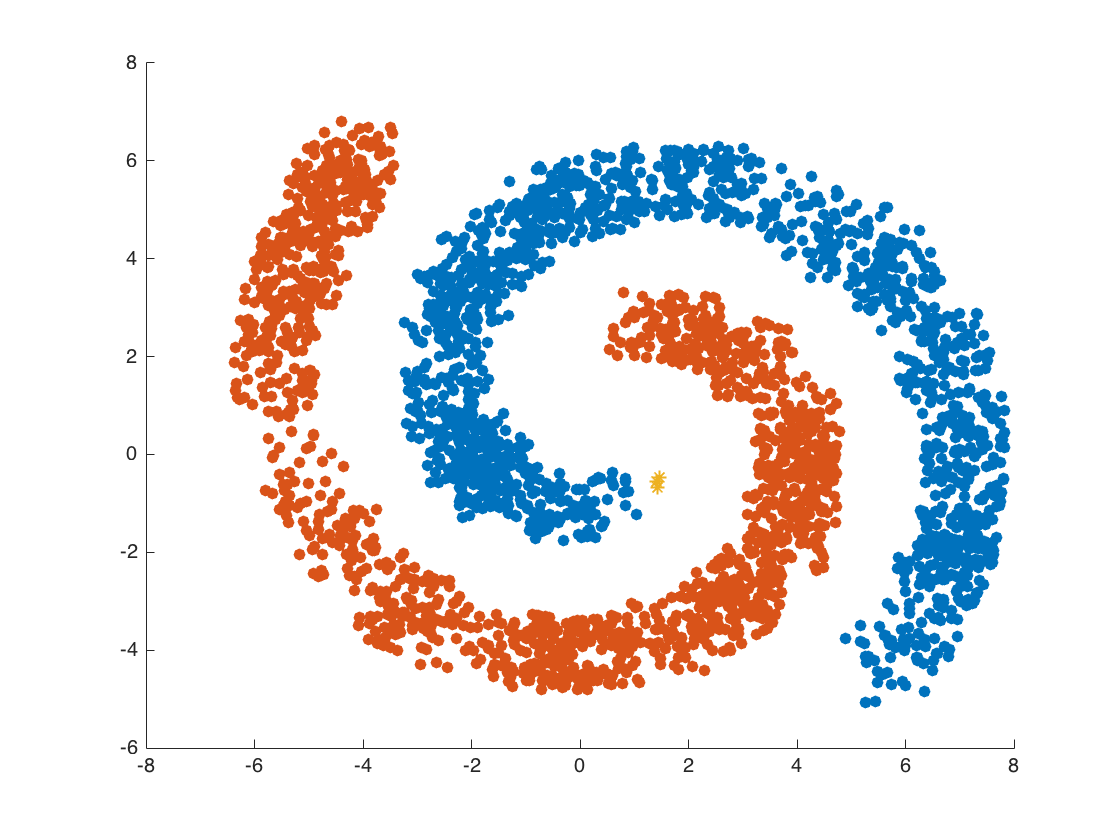
\includegraphics[scale=0.18]{img/dbscan.png}
                    \caption{DBSCAN}
                \end{figure}
            
            \vspace*{2mm}
            \subsubsection{Objetivo}

                Como objetivo, queremos encontrar un conjunto de agrupaciones que logre encapsular las posibles diferencias entre los pacientes. Como resultados esperaríamos ver que este algoritmo encuentre un cluster para cada uno de los niveles de riesgo de cáncer que definimos con anterioridad.
            
            \vspace*{2mm}
            \subsubsection{Implementación}

                Para nuestra implementación hemos usado la librería \emph{scikit-learn} \cite{scikit-learn}, a través de su API hemos entrenado varias instancias de un DBSCAN, en cada uno de ellos hemos variado el parámetro $\epsilon$ o (min\_distance). Para cada uno de los modelos hemos graficado su \emph{Silhouette Score}, el número de clusters que encuentran, y cuantas instancias pertenecen a cada cluster. Al final hemos escogido el modelo con un Silhouette Score aceptable que encuentra un número de clusters igual a los diferentes niveles de riesgo de tener cáncer que definimos en nuestra entrega anterior
    
    \vspace*{2mm}
    \section{Resultados} \label{resultados}
        
        Cada uno de los métodos implementados fue probado con la función mágica de \emph{Jupyter}, \emph{timeit}. A excepción del dendrograma, obtuvimos métricas del tiempo de entrenamiento y el puntaje silhouette.
        
        \begin{center}
            \begin{tabular}{|c|c|c|}
                \hline
                Modelo & Tiempo & Silhouette Score \\
                \hline
                K-Means & 2.7 s & 0.6119 \\
                \hline
                Dendrograma & - & - \\
                \hline
                Spectral Clustering & 31.2 ns & 0.5847 \\
                \hline
                DBSCAN & 461 ms & 0.2613 \\
                \hline
            \end{tabular}
        \end{center}
    
    \vspace*{4mm}    
    \section{Conclusiones} \label{conclusiones}
        
        \subsection{Áreas de mejora} \label{improvements}
        
            La complejidad de los modelos implementados en esta entrega volvió algo difícil que pudiéramos medir el desempeño de los algoritmos, y dada también la complejidad de la base de datos (datos médicos con alta correlación), es difícil que un algoritmo de agrupamiento tenga un desempeño ejemplar sin hacer un estudio mucho más detallado de los datos.
            
            De momento el área de mejora que hemos encontrado está enfocada al tiempo, procesamiento e interpretación del dendrograma. A diferencia de los demás modelos, crear un dendrograma y visualizarlo dentro de nuestro IDE fue una tarea lenta. Una vez que se tuvo un resultado, fue difícil implementar los datos generados, consideramos que esta opción no es viable cuando se tiene un alto volumen de datos.
            
        \subsection{Modelo seleccionado} \label{selected-model}
            
            El mejor modelo que encontramos fue el \emph{spectral-clustering}. Su puntaje silhouette se situó por debajo del obtenido por \emph{kmeans}, pero su tiempo de entrenamiento es 9 órdenes de magnitud menor al de \emph{kmeans}.
    
    \vspace*{4mm}        
    \section{Reflexiones} \label{thoughts}
    \vspace*{2mm}
    
        \subsection{Grace Aviance Silva Aróstegui}
        
            Con este trabajo me di cuenta de que los algoritmos de Aprendizaje No Supervisado son complicados para que se pueda realizar un buen análisis de la información y categorización. No porque sea malo este tipo de algoritmos o deficientes en calidad. Sin embargo, en comparación con el de Aprendizaje Supervisado el cual si tiene las categorías en los datos; el hecho de que el No Supervisado no tenga las categorías especificadas como el Supervisado (lo cual es característico del algoritmo) hace que no sea sencillo analizar cualquier base de datos. Y esto lo podemos observar sobretodo en el Dendrograma, con todo tan caótico no es realmente práctico hacer este tipo de análisis para principantes por ejemplo, es decir, se necesita mucho conocimiento y habilidades para poder sacarle gran provecho a estos tipos de algoritmos.
        
        \subsection{Emily Rebeca Méndez Cruz}
        
            Gracias a este trabajo he podido darme cuenta de lo complicado que es la ciencia de datos, pero también de lo interesante que es. Los algoritmos no supervisados se me hicieron un modelo algo complicado de entender pero atrayentes. Son una manera en la que podemos agrupar nuestra base de datos cuando no se quiere hacer un entrenamiento a este, es decir, cuando se parte de datos no etiquetados previamente para que el algoritmo intente entenderlo por sí mismo. Lo complicado de esta actividad es que no contamos con el conocimiento necesario para generar un mejor modelo, ni el equipo.
        
        \subsection{Juan Pablo Echeagaray González}

            Los algoritmos de aprendizaje no supervisados son en verdad bastante interesantes. Me sorprendió mucho lo diferentes que pueden ser de los algoritmos discutidos con anterioridad. Una de las principales dificultades a las que me enfrenté fue decidir como medir el desempeño de cada uno de los modelos; descartando el tiempo de entrenamiento, creo que es muy complicado que un científico de datos por sí solo pueda medir qué tan bien funciona un modelo aplicado a un área tan compleja y crítica como lo es la medicina.
        
    \appendices
    
    \section{Datos} \label{data}

        Base de datos consistente de 36 características y de 858 observaciones. Está compuesta principalmente de variables categóricas que indican si alguna enfermedad o afección se encontró presente en el individuo. Consta de pocas variables numéricas como lo son la edad, el número de embarazos y de parejas sexuales, la edad en la que se tuvo la primera relación sexual y el número de años que ha fumado.

        Los datos usados en este proyecto pueden descargarse \href{https://www.kaggle.com/code/ravaliraj/risk-classification-of-cervical-cancer}{aquí}.

    \section{Código} \label{code}

        El código desarrollado se encuentra en el siguiente \href{https://github.com/JuanEcheagaray75/cancer-clf}{repositorio}

    \section{Evidencias de trabajo en equipo}
    \begin{figure}[!ht]
        \centering
        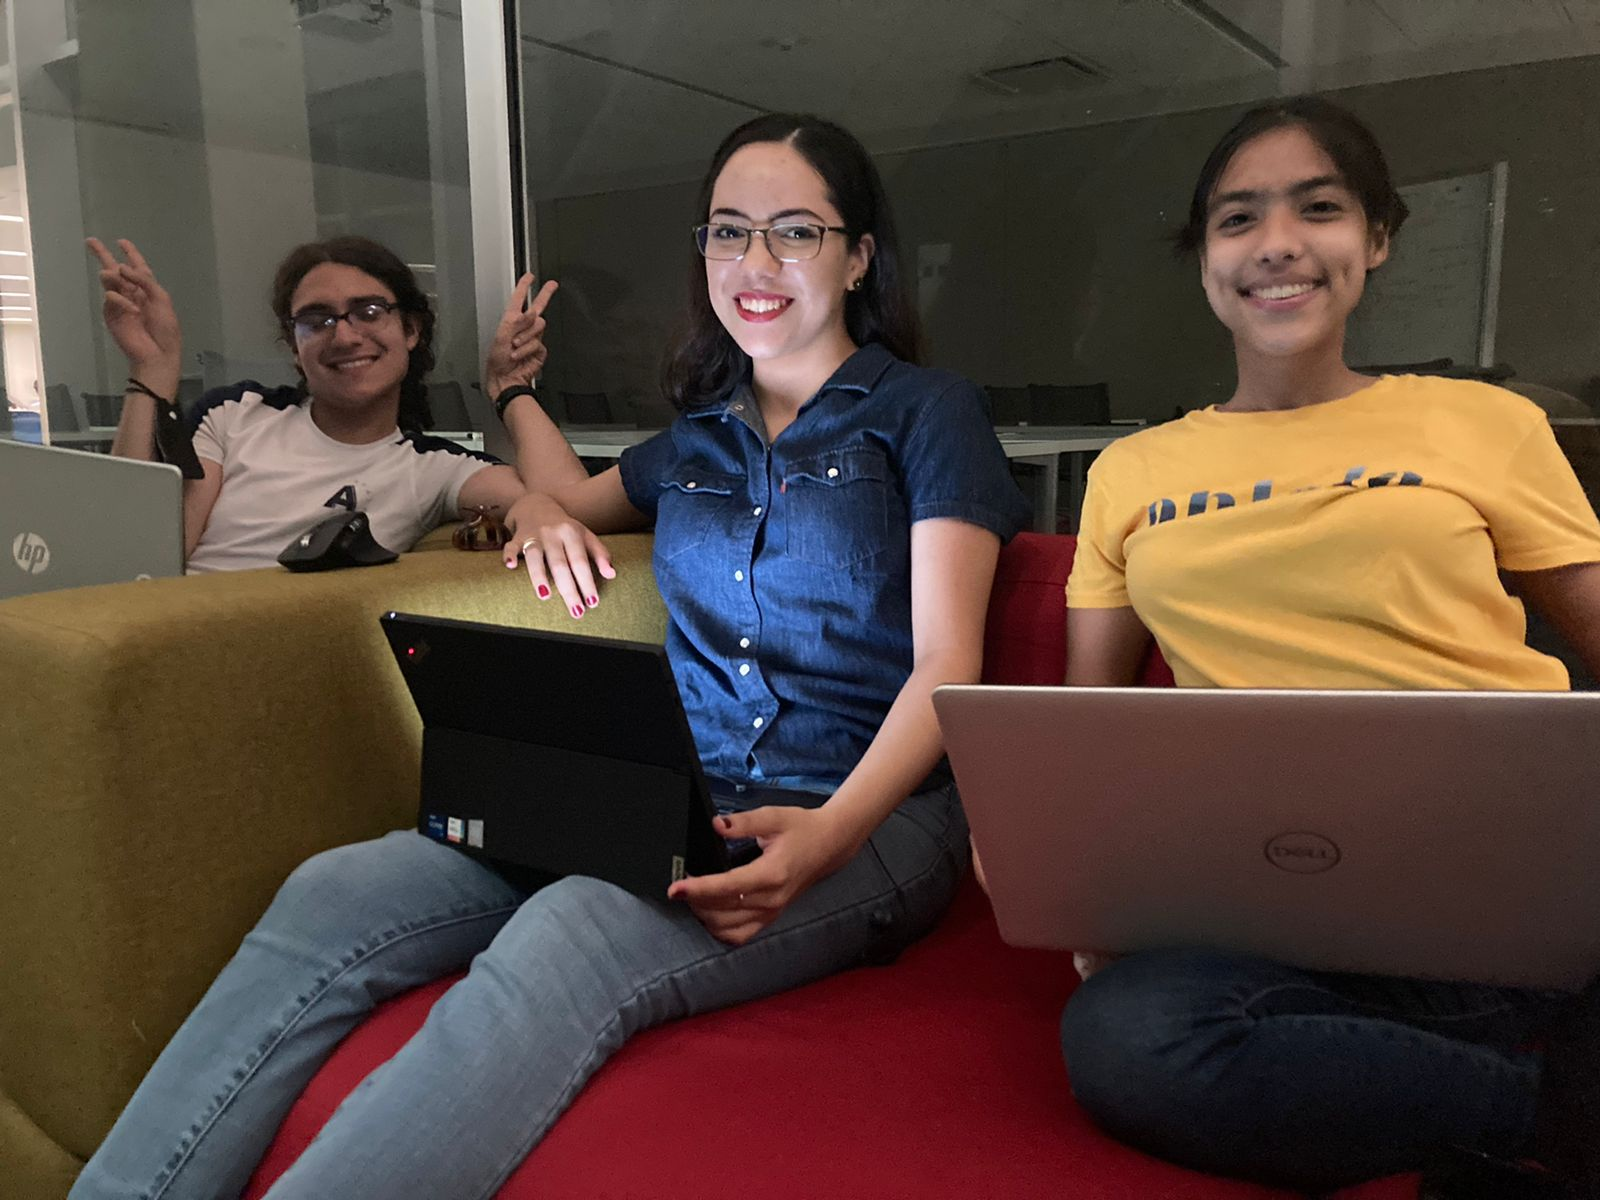
\includegraphics[scale=0.1]{img/team.jpg}
    \end{figure}


    \bibliographystyle{IEEEtran}
    \bibliography{references.bib}

\end{document}